%%==================================================
%% chapter01.tex for BIT Master Thesis
%% modified by pinren lu
%% version: 0.1
%% last update: Dec 25th, 2016
%%==================================================
% 第五章 模型改写文本检测系统设计与实现

% 1. 需求分析
% 2. 系统设计
% 3. 系统实现
% 4. 系统展示
% 5. 本章小结

\chapter{模型改写文本检测系统设计与实现}
\label{chap:sys}

本章主要介绍基于模型改写文本检测系统的设计与实现,第三、四章从理论和实验方面验证了本文提出方法的有效性,为了进一步验证方法在实际应用场景中的有效性,本文以提出的模型改写文本检测方法为基础,遵循软件开发过程的基本原则,设计并实现了模型改写文本检测系统,涵盖文本改写和检测模型改写两大文本生成功能。通过该系统,可以进一步提升文本改写的流畅性与多样性、检测模型改写的准确性。本章以需求分析、系统设计、系统实现以及系统功能展示四个部分介绍模型改写文本检测系统。

\section{需求分析}
\label{sec:sys-need}

本研究所提出的模型改写文本检测系统为自然语言处理领域提供了一种创新的技术解决方案,显著增强了对学生写作文本是否经过AI改写的检测能力。该系统旨在为用户提供一个功能全面、性能卓越的文本改写检测平台,能够满足多样化的文本改写需求,并提供精准的模型文本改写检测服务。接下来,将从业务需求和功能需求的角度对该系统进行详细分析。

\subsection{业务需求分析}
\label{sec:sys-bus-need}

随着人工智能技术的迅速进步,文本改写及其检测的需求日益增加。尤其在教育领域,教师迫切需要评估和反馈学生的写作,而学生则希望借助改写工具来提升自己的写作能力。因此,本文提出的模型改写文本检测系统应满足以下业务需求:

(1)\textbf{高质量文本改写服务:} 系统应能够提供优质的文本改写服务,以帮助用户提升文本的流畅性和多样性;
(2)\textbf{准确的模型改写检测服务:} 系统应具备准确识别文本是否经过模型改写的能力,以便教师有效评估学生的写作水平;
(3)\textbf{用户友好的界面设计:} 系统应提供简洁明了的用户界面,以便用户轻松操作;
(4)\textbf{卓越的性能与稳定性:} 系统应具备出色的性能和稳定性,以处理大量文本数据;
(5)\textbf{数据安全与隐私保护:} 系统应确保用户数据的安全性,并提供隐私保护措施,以防止数据泄露;
(6)\textbf{良好的可扩展性:} 系统应具备良好的可扩展性,以支持根据需求进行功能的扩展与升级;
(7)\textbf{多平台兼容性:} 系统应能够在多种平台上运行,包括桌面和移动设备;
(8)\textbf{实时反馈机制:} 系统应提供实时的文本改写与检测反馈,帮助用户及时了解文本质量和改写效果;
(9)\textbf{用户管理功能:} 系统应具备用户管理功能,支持用户注册、登录及权限管理等操作。

\subsection{功能需求分析}
\label{sec:sys-func-need}

本文从用户与管理员两个视角对系统功能进行了全面分析,以深入理解不同用户身份下的需求与功能要求。在用户功能需求分析中,重点关注系统所提供的各项服务与功能,包括用户注册、登录、文本改写和检测功能,以及用户历史信息的管理。这些功能旨在确保用户能够顺利使用系统并获得良好的使用体验。在管理员功能需求分析方面,重点则放在系统的管理与维护功能上,包括用户管理、功能管理、模型管理以及文本改写信息的管理。这些功能的设计旨在确保系统高效、稳定地运行,并能够及时处理用户反馈与相关问题。通过这样的分析,能够更全面地满足不同用户群体的需求。

\begin{figure*}[htb]
    \centering
    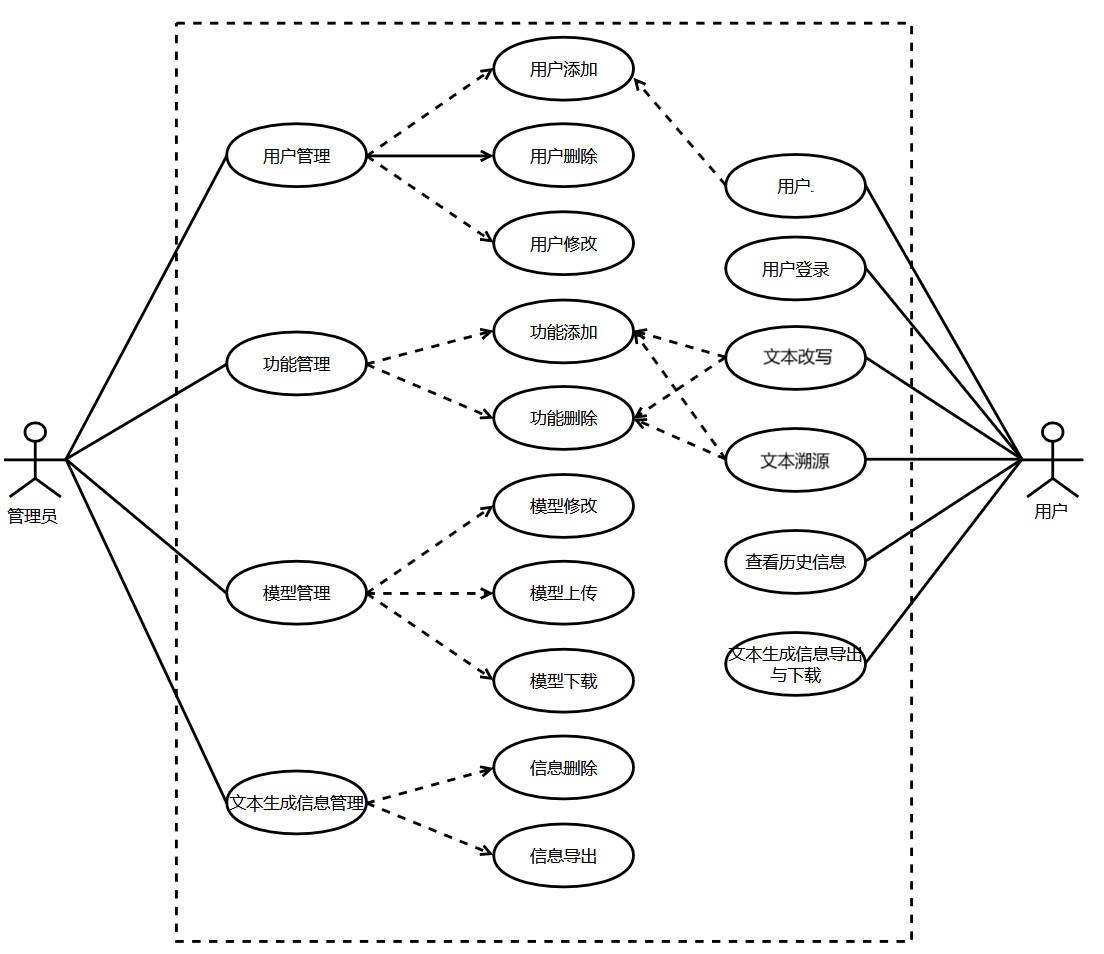
\includegraphics[width=\textwidth]{figures/sys-use-case.jpg}
    \caption{模型改写文本检测系统用例图}
    \label{fig:sys-use-case}
\end{figure*}

模型改写文本检测系统的总体用例图如图 \ref{fig:sys-use-case} 所示。

本系统的用户功能需求分析如下:

(1)\textbf{用户注册}:系统允许用户自主进行注册,以便创建个人账户;(2)\textbf{用户登录}:用户可凭借已注册的账号和密码成功登录系统;(3)\textbf{文本改写服务}:系统应为用户提供文本改写服务,能够根据用户输入的文本进行润色,使其更加流畅和通顺;(4)\textbf{文本溯源服务}:系统应提供检测服务,以判断某段文本是否经过改写或由人工智能生成,依据输入的源文本得出相应的检测结果;(5)\textbf{查看历史信息}:用户可以通过历史信息查询接口查看以往的改写记录和检测结果;(6)\textbf{文本生成信息导出与下载}:支持用户将文本信息导出并下载至本地存储。

本系统的管理员功能需求分析如下:

(1)\textbf{用户管理}:管理员可对用户进行添加、删除及信息修改等管理操作;
(2)\textbf{功能管理}:系统支持功能的扩展,允许管理员添加新功能或删除不必要的功能;
(3)\textbf{模型管理}:管理员可以通过模型管理接口进行模型的修改、上传和下载;
(4)\textbf{文本生成信息管理}:管理员负责对系统内冗余的文本信息进行删除或导出操作。

\section{系统设计}
\label{sec:sys-design}

本章主要介绍模型改写文本检测系统的架构设计、模块和接口设计以及相关信息的数据库存储设计。

\subsection{系统架构设计}
\label{sec:sys-arch}

为增强系统的灵活性、可扩展性与可维护性,本系统采用了前后端分离的架构设计。在该架构中,前端主要负责接收用户输入数据并发送相应的系统反馈,而后端则承担具体的服务提供和处理逻辑,并将处理结果反馈至前端。系统的整体架构如图 \ref{fig:sys-arch} 所示,涵盖表现层、应用层、持久层及基础层。

\begin{figure*}[htb]
    \centering
    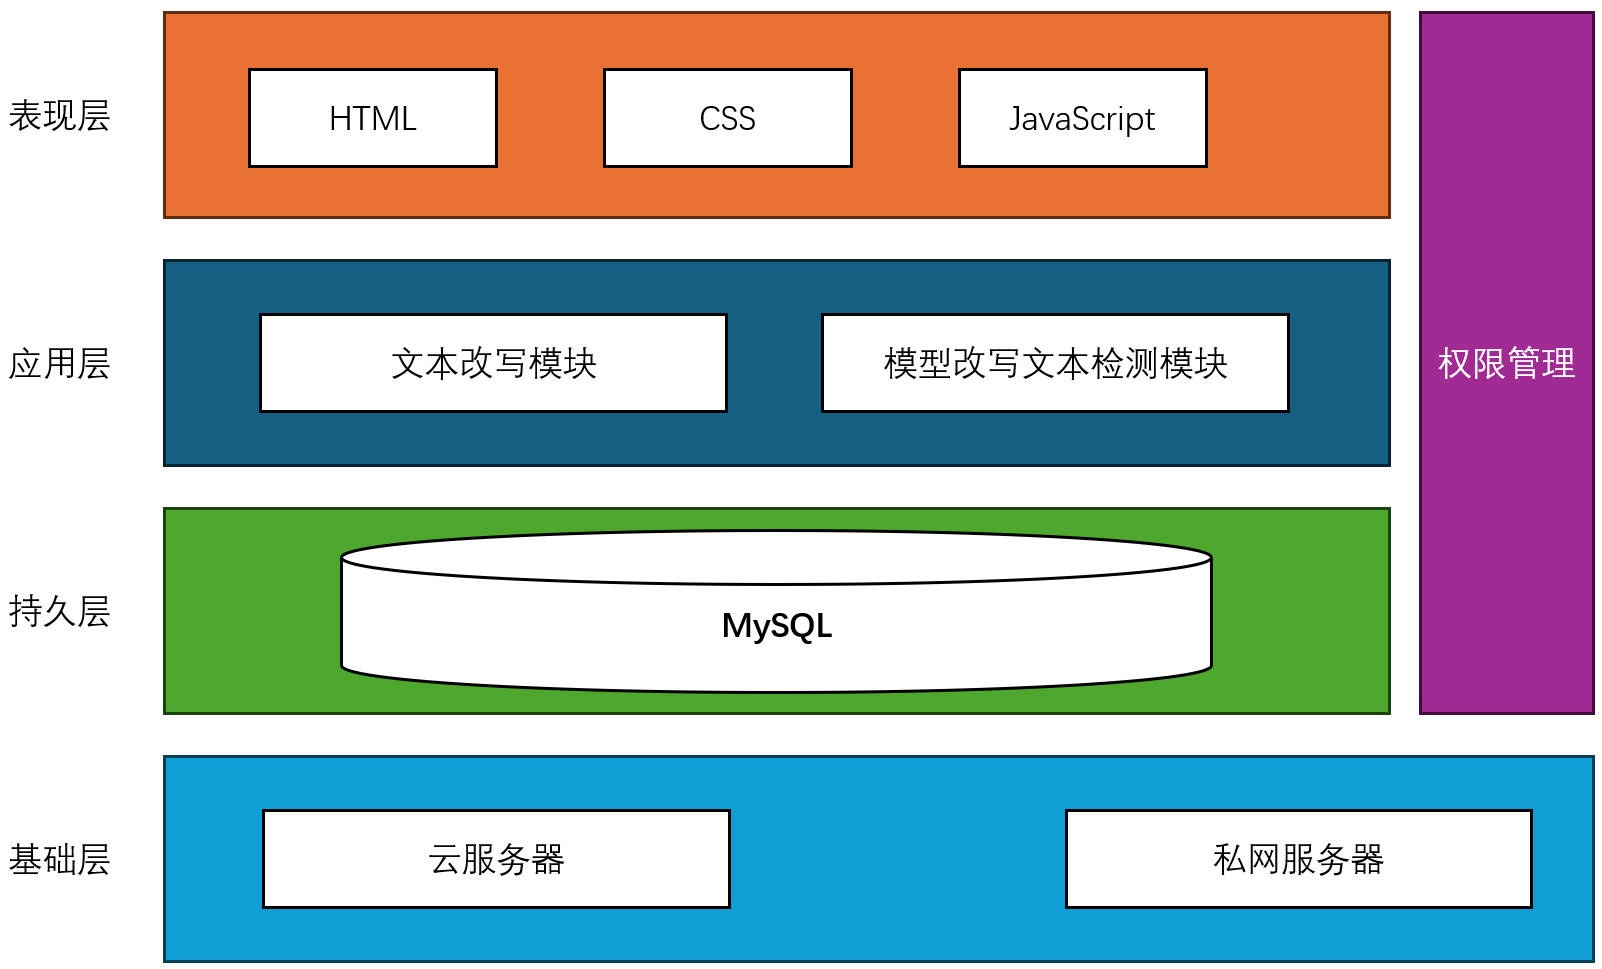
\includegraphics[width=\textwidth]{figures/sys-architecture.jpg}
    \caption{模型改写文本检测系统架构设计}
    \label{fig:sys-arch}
\end{figure*}

(1)\textbf{表现层}:该层负责处理用户界面的逻辑与交互控制,管理界面的逻辑和权限设置,以用户友好的方式展示系统数据并实现用户交互。其内容涵盖用户界面设计、页面布局及组件设计、样式设计与美化。该层通过 HTML 定义页面结构,利用 CSS 进行样式美化,并通过 JavaScript 处理页面交互及动态效果。

(2)\textbf{应用层}:此层包含系统的核心业务逻辑,包括对话生成模块和机器翻译模块,同时提供用户管理及管理员管理服务。将业务逻辑独立设置于应用层,有助于不同功能模块的开发、测试和部署的独立性与灵活性,从而便于后续功能的扩展与升级。

(3)\textbf{持久层}:该层负责系统的数据存储与访问管理,使用 MySQL 存储用户账户信息、个人资料、权限与角色信息以及用户活动记录等结构化数据。同时,利用 MongoDB 存储生成的文本内容等非结构化信息。通过独立的数据层,系统的数据访问变得更加统一与安全,同时也便于数据的管理与维护。

(4)\textbf{基础层}:该层通过云服务器和私有网络服务器进行系统部署,提供必要的基础运行环境。

通过采用前后端分离的系统架构,本系统能够实现前后端的松耦合、功能模块化
和独立部署,提高了系统的灵活性、可扩展性和可维护性,同时也提高了开发效率。

\subsection{模块和接口设计}
\label{sec:sys-module}

模型改写文本检测系统的结构可分为用户模块、系统管理模块和系统功能模块
% ,模块之间的关系如图 \ref{fig:sys-module} 所示
。用户模块的主要功能包括用户的注册与登录,允许用户创建账户、进行密码管理,并提供身份验证与授权功能,以确保用户能够顺利访问和使用系统服务。系统管理模块则专注于功能管理、模型管理和数据管理,支持对系统功能的灵活扩展,管理员可以通过该模块添加新功能或移除不再需要的功能。此外,模型管理接口允许对系统模型进行修改、上传和下载,而数据管理功能则负责管理文本生成信息,用户可以通过系统接口删除冗余文本信息或将其导出至本地。系统功能模块是系统的核心部分,提供多种具体的系统服务,以处理前端接收的请求。系统功能涵盖文本改写和文本检测等,通过此模块,用户可以与系统进行交互,发起特定请求或执行特定任务。系统根据接收到的请求,调用相应的功能模块进行处理,并生成相应的响应。

% \begin{figure*}[htb]
%     \centering
%     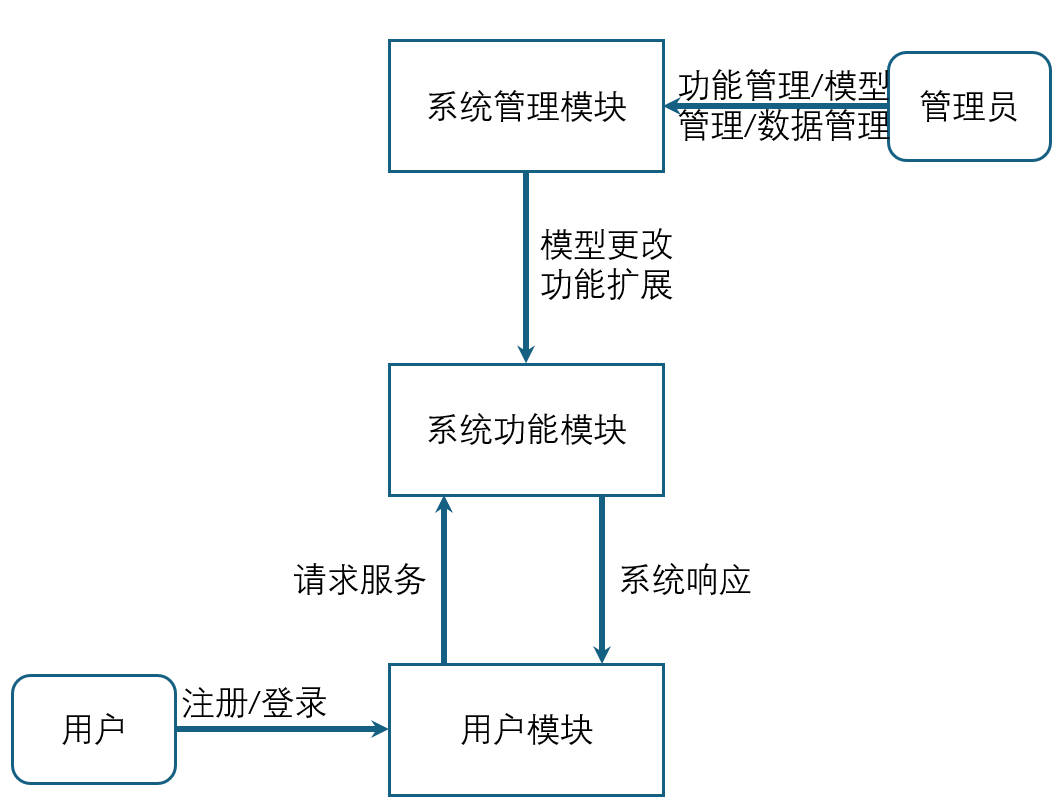
\includegraphics[width=0.8\textwidth]{figures/sys-module.jpg}
%     \caption{模型改写文本检测系统模块设计}
%     \label{fig:sys-module}
% \end{figure*}

为了实现系统对用户的服务以及系统内不同模块之间数据传输,本章定义了系统核心接口,如表 \ref{tab:sys-interfaces} 所示,其中展示了模型改写文本检测系统核心接口及所属模块。

\begin{table*}[htb]
    \centering
    \caption{模型改写文本检测系统核心接口及所属模块说明}
    \label{tab:sys-interfaces}
    \begin{tabular}{ccl}
        \toprule
        \textbf{接口名} & \textbf{所属模块} & \textbf{接口描述} \\
        \midrule
        userRegister & 用户模块 & 接收用户提交注册信息,并进行用户注册。 \\
        userLogin & 用户模块 & 接收用户提交登录信息,并进行身份验证和授权。 \\
        getModelInfo & 系统管理模块 & 查询系统提供的模型,返回相关模型信息。 \\
        upLoadModel & 系统管理模块 & 用于上传已训练好的模型到系统中,以供后续的服务需求。 \\
        downLoadModel & 系统管理模块 & 用于从系统中导入已有模型。 \\
        funcDelete & 系统管理模块 & 用于删除系统中不需要的功能。 \\
        funcCreate & 系统管理模块 & 用于扩展系统功能,提供更好的服务。 \\
        dataManage & 系统管理模块 & 用于管理系统中的文本生成信息,支持删除或下载文本数据。 \\
        polishService & 系统功能模块 & 接收用户输入,使用模型进行文本改写,并返回结果。 \\
        detectService & 系统功能模块 & 接收用户输入,使用模型进行模型改写文本检测,并返回结果。 \\
        \bottomrule
    \end{tabular}
\end{table*}

\subsection{数据库设计}
\label{sec:sys-db}

根据系统的存储需求,本文选择使用 MySQL 数据库来存储结构化数据,具体包括用户表、功能表、模型表和文本数据表等。

MySQL 数据库的设计主要涵盖用户表、功能表、模型表以及文本数据表。每个表均设有相应的字段和数据类型,以满足系统的特定需求。

用户表用于记录用户的相关信息,包括用户 ID、用户名、密码、邮箱、权限、注册时间以及最近登录时间等,具体结构如表 \ref{tab:user-table} 所示。

\begin{table*}[htb]
    \centering
    \caption{用户表} \label{tab:user-table}
    \begin{tabular}{ccccc}
        \toprule
        \textbf{序号} & \textbf{字段} & \textbf{数据类型} & \textbf{说明} & \textbf{是否主键} \\
        \midrule
        1 & user\_id & int & 用户 ID & 是 \\
        2 & user\_name & varchar(30) & 用户名 & 否 \\
        3 & password & varchar(128) & 密码 & 否 \\
        4 & email & varchar(30) & 邮箱 & 否 \\
        5 & authority & enum & 权限 & 否 \\
        6 & register\_time & datetime & 注册时间 & 否 \\
        7 & lat\_login\_time & datetime & 最近登录时间 & 否 \\
        \bottomrule
    \end{tabular}
\end{table*}

功能表用于记录系统中各项相关功能的信息,具体包括功能 ID、功能名称及其对应的功能接口,详细结构如表 \ref{tab:func-table} 所示。

\begin{table*}[htb]
    \centering
    \caption{功能表} \label{tab:func-table}
    \begin{tabular}{ccccc}
        \toprule
        \textbf{序号} & \textbf{字段} & \textbf{数据类型} & \textbf{说明} & \textbf{是否主键} \\
        \midrule
        1 & fuc\_id & int & 功能 ID & 是 \\
        2 & fuc\_name & varchar(30) & 功能名称 & 否 \\
        3 & fuc\_interface & varchar(30) & 功能接口 & 否 \\
        \bottomrule
    \end{tabular}
\end{table*}

模型表用于存储与系统内模型相关的信息,涵盖模型 ID、模型名称、模型类型以及模型的上传时间等内容。具体结构详见表 \ref{tab:model-table}。

\begin{table*}[htb]
    \centering
    \caption{模型表} \label{tab:model-table}
    \begin{tabular}{ccccc}
        \toprule
        \textbf{序号} & \textbf{字段} & \textbf{数据类型} & \textbf{说明} & \textbf{是否主键} \\
        \midrule
        1 & model\_id & int & 模型 ID & 是 \\
        2 & model\_name & varchar(20) & 模型名称 & 否 \\
        3 & model\_type & varchar(20) & 模型类型 & 否 \\
        4 & model\_size & varchar(20) & 模型大小 & 否 \\
        5 & upload\_time & datetime & 上传时间 & 否 \\
        \bottomrule
    \end{tabular}
\end{table*}

文本数据表旨在记录与用户及模型改写文本相关的信息,具体包括用户 ID、文本 ID、操作类型、操作时间以及文本内容等。该表的详细结构如表 \ref{tab:text-table} 所示。

\begin{table*}[htbp]
    \centering
    \caption{文本数据表} \label{tab:text-table}
    \begin{tabular}{ccccc}
        \toprule
        \textbf{序号} & \textbf{字段} & \textbf{数据类型} & \textbf{说明} & \textbf{是否主键} \\
        \midrule
        1 & user\_id & int & 用户 ID & 是 \\
        2 & text\_id & int & 文本 ID & 是 \\
        3 & text\_type & varchar(20) & 操作类型 & 否 \\
        4 & generated\_time & datetime & 操作时间 & 否 \\
        5 & text\_content & text & 文本内容 & 否 \\
        \bottomrule
    \end{tabular}
\end{table*}

\section{系统实现}
\label{sec:sys-implement}

本节将详细介绍模型改写文本检测系统所使用的工具和系统服务,并对系统功能进行模块化阐述。

\subsection{开发环境与工具}
\label{sec:sys-env}

本研究采用前后端分离的架构进行系统开发。前端部分利用 Vue 框架构建用户界面,以提供优良的交互体验。后端则基于 Pytorch 和 Transformers 等技术,负责文本生成服务的构建。在编程语言的选择上,前端和后端分别使用 HTML、CSS、JavaScript 和 Python,以满足不同开发需求。为提升开发效率,选用 Vscode 作为主要开发工具。在数据存储方面,系统采用 MySQL 数据库,以存储用户信息及生成的文本数据。为简化后端业务逻辑的处理,使用 Flask 框架。此外,为确保系统的安全性,采用 JWT 技术进行权限管理和用户身份验证。本文所使用的所有开发环境和工具的详细信息见表 \ref{tab:sys-env}。

\begin{table*}[htbp]
    \centering
    \caption{模型改写文本检测系统开发环境与工具}
    \label{tab:sys-env}
    \begin{tabular}{cc}
        \toprule
        \textbf{描述} & \textbf{配置} \\
        \midrule
        编程语言 & HTML、CSS、JavaScript、Python \\
        前端框架 & Vue \\
        服务端开发 & Pytorch1.8、Transformers \\
        开发工具 & Vscode \\
        数据库 & MySQL \\
        权限管理 & JWT \\
        服务器端 & Flask1.1.2、Docker \\
        \bottomrule
    \end{tabular}
\end{table*}

鉴于管理员仅能在系统后台通过脚本执行管理操作,本文将重点展示用户端的系统功能。用户端主要包括用户注册与登录、文本改写、检测模型改写以及历史信息查询等功能。用户注册与登录功能旨在允许用户创建账户并访问系统;文本改写功能则用于对用户输入的文本进行改写;检测模型改写功能用于验证输入文本是否经过模型处理;历史信息查询功能则帮助用户检索其过往操作记录。

\subsection{用户注册与登录}

用户可以通过已注册的账号和密码登录系统,相关界面如图 \ref{fig:sys-login} 所示。在用户注册过程中,需填写用户名、密码和电子邮箱等信息,系统将对所输入的信息进行验证,以确保其合法性和完整性。如果用户尚未注册账户,可以通过注册页面进行注册,具体界面如图 \ref{fig:sys-register} 所示。

\begin{figure*}[htb]
    \subfloat[listentry][用户登录]{
        \label{fig:sys-login}
        \centering
        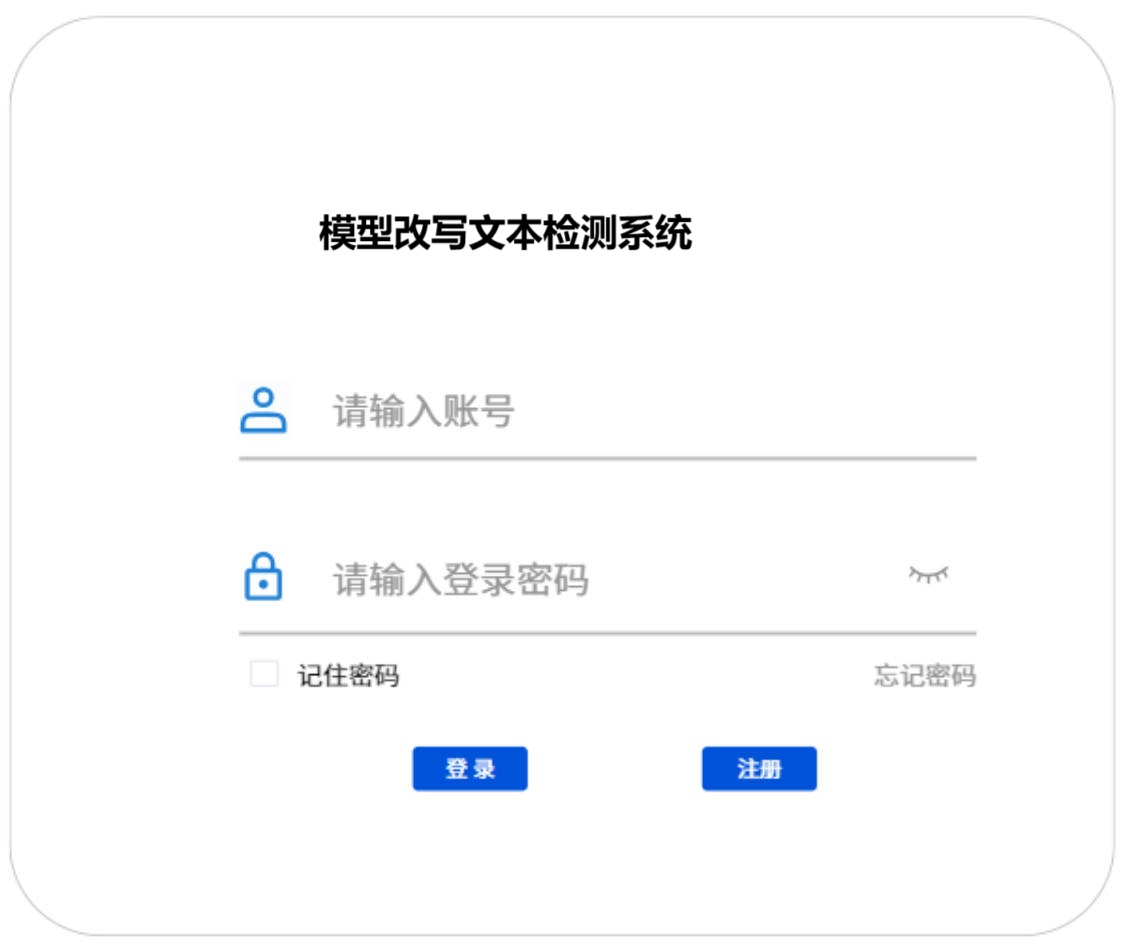
\includegraphics[width=0.45\textwidth]{figures/sys-login.jpg}
    }
    \hfill
    \subfloat[listentry][用户注册]{
        \label{fig:sys-register}
        \centering
        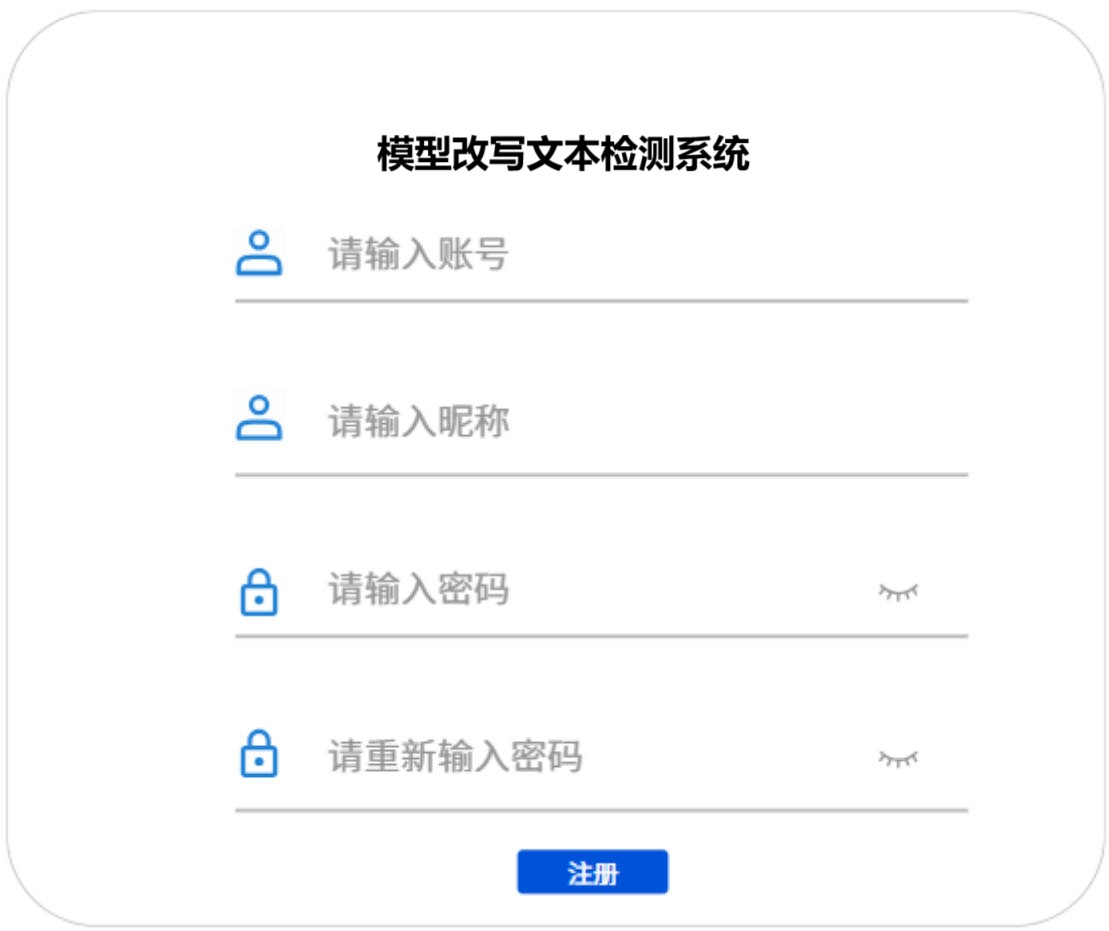
\includegraphics[width=0.45\textwidth]{figures/sys-register.jpg}
    }
    \caption{模型改写文本检测系统用户注册与登录}
    \label{fig:sys-login-register}
\end{figure*}

\subsection{文本改写功能}

用户成功登录系统后,可以进行文本改写操作,具体界面如图 \ref{fig:sys-polish} 所示。在此过程中,用户需输入待改写的文本,系统将利用相应的模型进行处理,并返回改写后的结果。用户可以查看并下载生成的文本。此外,系统允许用户选择不同的改写模型,以便进行针对性的文本处理。用户也可以对改写后的文本进行进一步编辑和修改,以满足个人需求。

\begin{figure*}[htb]
    \centering
    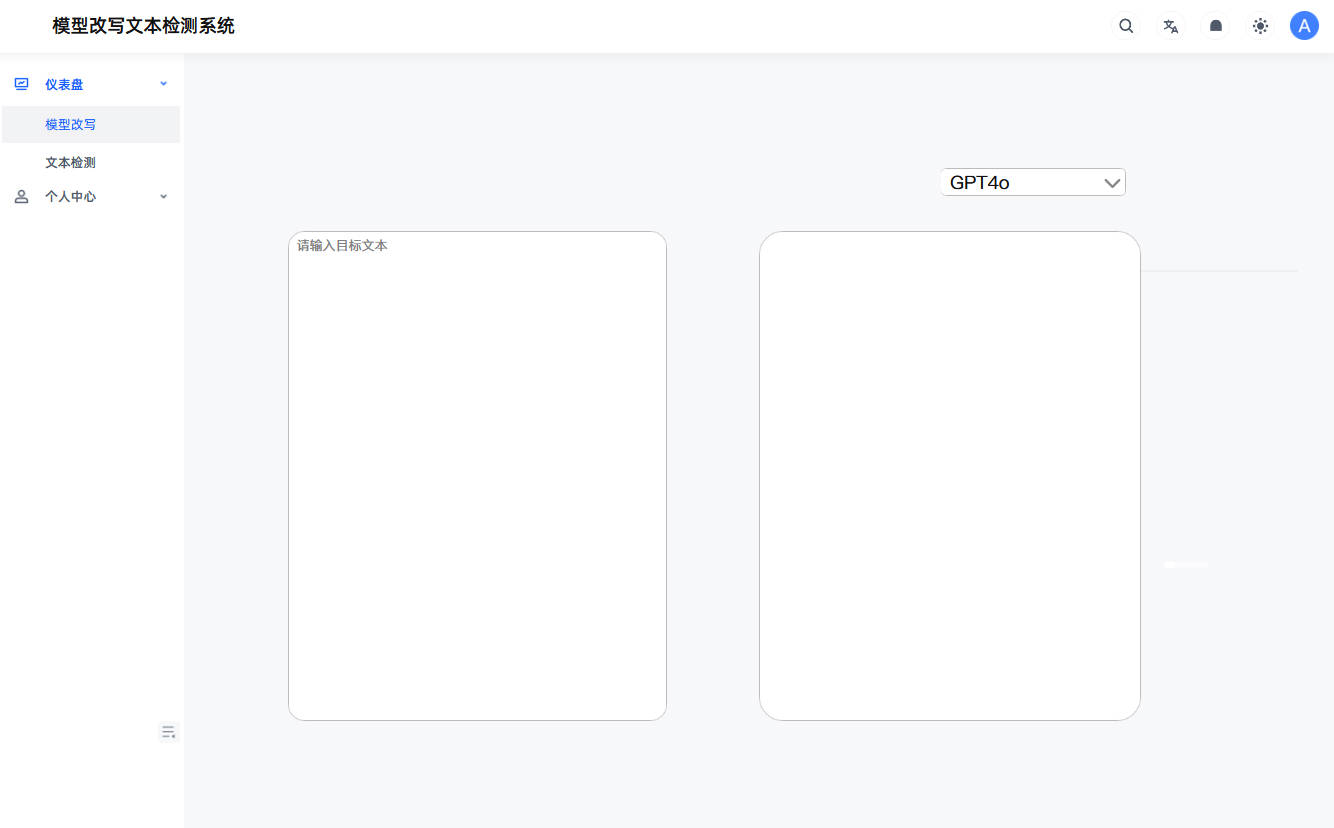
\includegraphics[width=\textwidth]{figures/sys-polish.jpg}
    \caption{模型改写文本检测系统——文本改写功能}
    \label{fig:sys-polish}
\end{figure*}

\subsection{模型改写文本检测功能}

在用户成功登录后,系统提供了模型改写文本检测的功能,具体界面如图 \ref{fig:sys-detect} 所示。用户可以输入待检测的文本,系统将运用相应的模型进行分析,并返回检测结果,检测后结果如图 \ref{fig:sys-detect2} 所示。用户有权查看并下载这些检测结果。此外,系统允许用户在后台选择不同的检测模型,以便为文本检测提供更为精确的处理,系统将依据用户的选择执行相应的操作。

\begin{figure*}[htb]
    \centering
    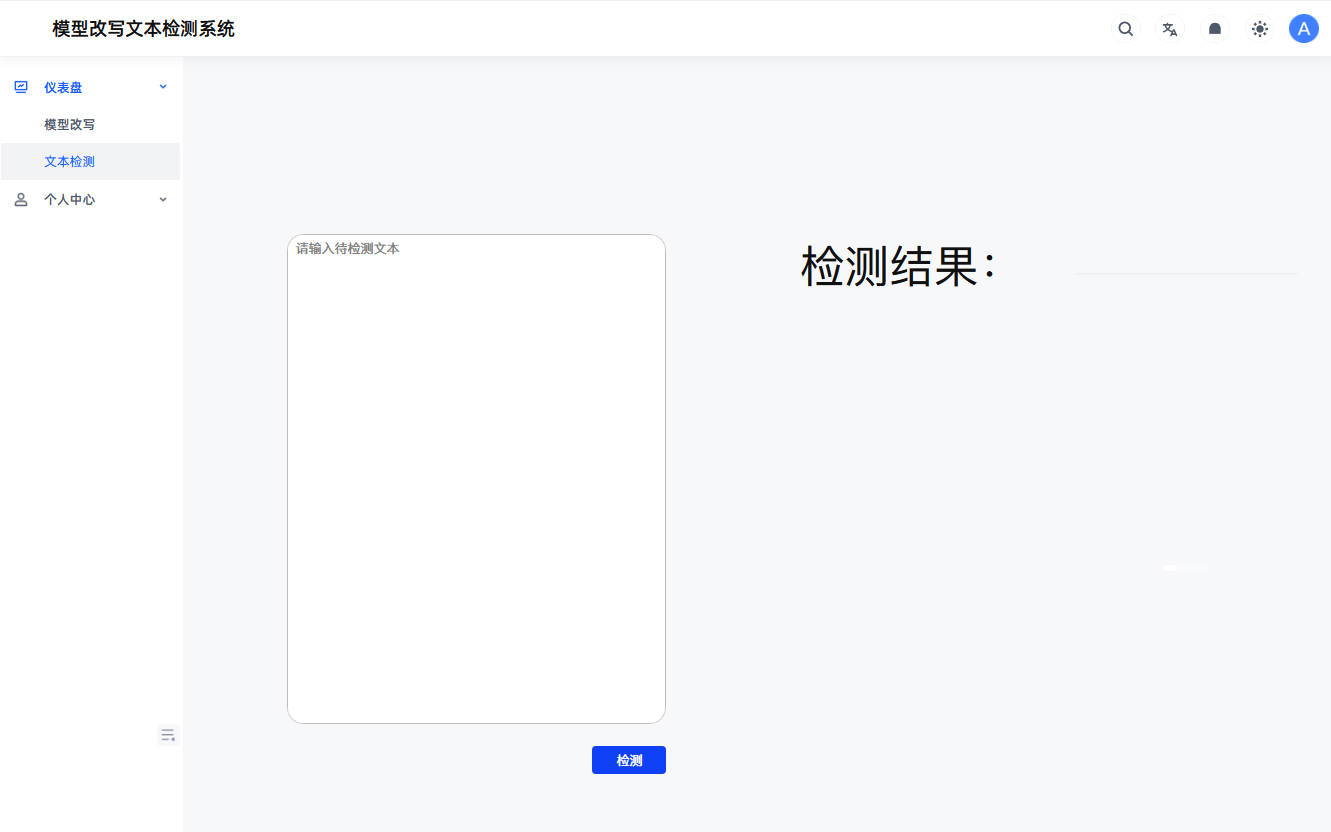
\includegraphics[width=\textwidth]{figures/sys-detect.jpg}
    \caption{模型改写文本检测系统——模型改写文本检测功能——检测前}
    \label{fig:sys-detect}
\end{figure*}

\begin{figure*}[htb]
    \centering
    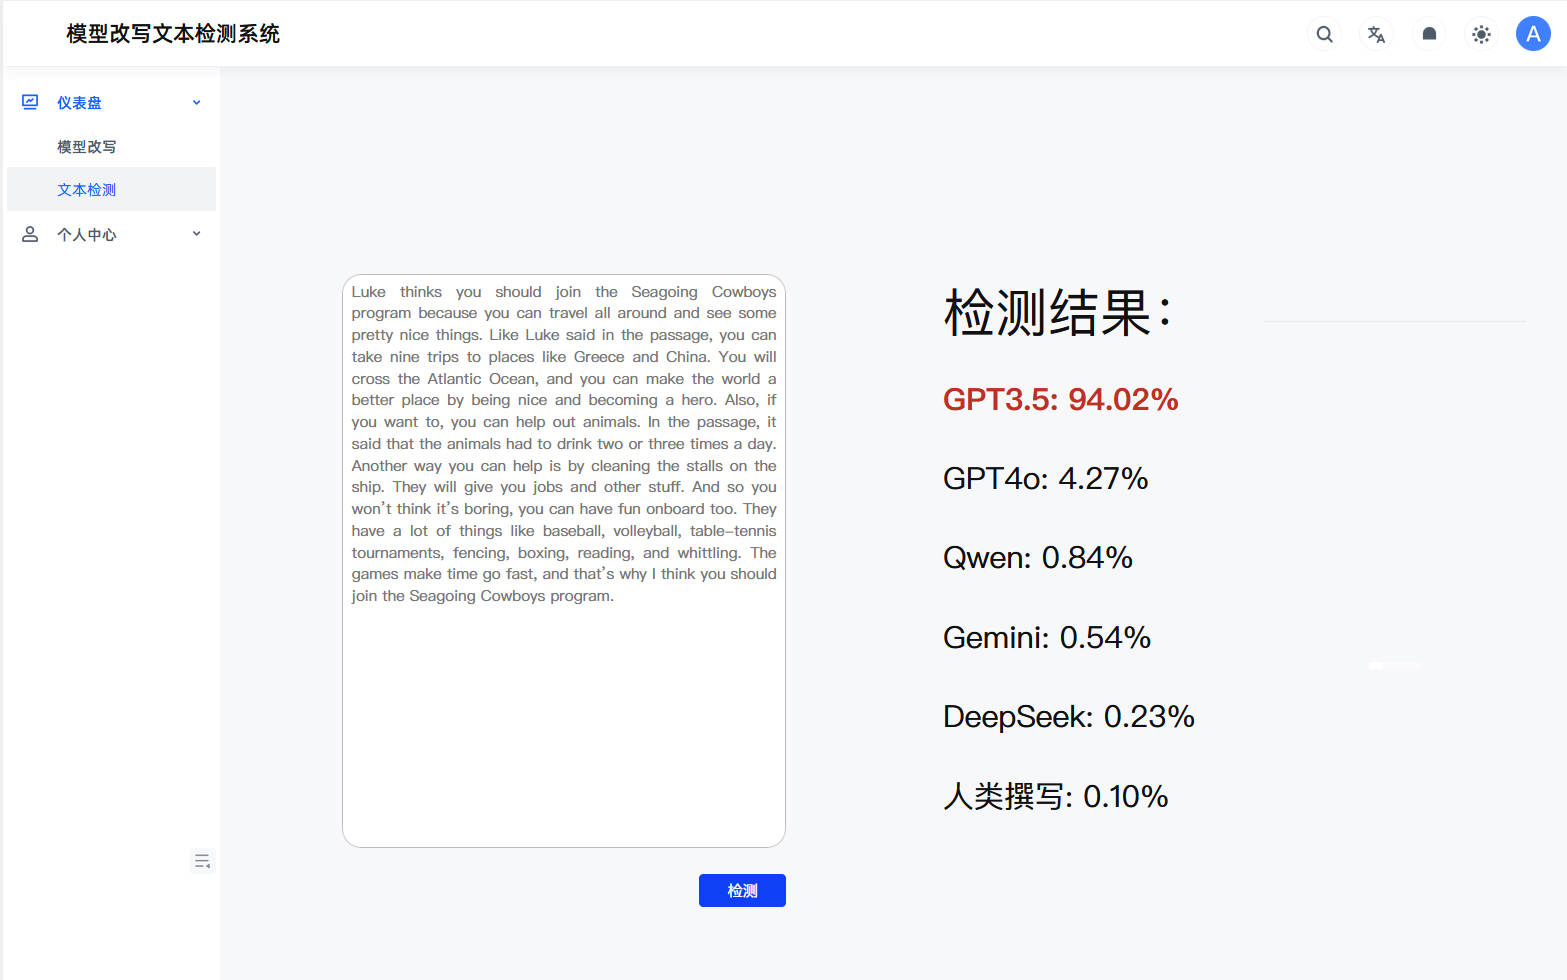
\includegraphics[width=\textwidth]{figures/sys-detect2.jpg}
    \caption{模型改写文本检测系统——文本改写功能——检测后}
    \label{fig:sys-detect2}
\end{figure*}

\section{本章小结}
\label{sec:sys-conclusion}

本章主要介绍了模型改写文本检测系统的设计与实现,包括需求分析、系统架构设计、模块和接口设计以及数据库设计。通过对系统的功能进行详细分析,明确了系统的业务需求和功能需求,为后续的系统实现提供了基础。系统采用前后端分离的架构设计,提高了系统的灵活性和可扩展性。通过模块和接口设计,明确了系统各个模块之间的关系和数据传输方式。数据库设计则为系统的数据存储提供了支持。最后,通过用户注册与登录、文本改写功能、模型改写文本检测功能等展示了系统的实际应用效果。

本章为模型改写文本检测系统的设计与实现奠定了基础,为后续的系统测试和优化提供了依据。通过对系统的设计与实现,可以看出模型改写文本检测系统在实际应用中的可行性和有效性,为后续的研究和应用提供了参考。